% GNUPLOT: LaTeX picture with Postscript
\begingroup
  \makeatletter
  \providecommand\color[2][]{%
    \GenericError{(gnuplot) \space\space\space\@spaces}{%
      Package color not loaded in conjunction with
      terminal option `colourtext'%
    }{See the gnuplot documentation for explanation.%
    }{Either use 'blacktext' in gnuplot or load the package
      color.sty in LaTeX.}%
    \renewcommand\color[2][]{}%
  }%
  \providecommand\includegraphics[2][]{%
    \GenericError{(gnuplot) \space\space\space\@spaces}{%
      Package graphicx or graphics not loaded%
    }{See the gnuplot documentation for explanation.%
    }{The gnuplot epslatex terminal needs graphicx.sty or graphics.sty.}%
    \renewcommand\includegraphics[2][]{}%
  }%
  \providecommand\rotatebox[2]{#2}%
  \@ifundefined{ifGPcolor}{%
    \newif\ifGPcolor
    \GPcolortrue
  }{}%
  \@ifundefined{ifGPblacktext}{%
    \newif\ifGPblacktext
    \GPblacktextfalse
  }{}%
  % define a \g@addto@macro without @ in the name:
  \let\gplgaddtomacro\g@addto@macro
  % define empty templates for all commands taking text:
  \gdef\gplbacktext{}%
  \gdef\gplfronttext{}%
  \makeatother
  \ifGPblacktext
    % no textcolor at all
    \def\colorrgb#1{}%
    \def\colorgray#1{}%
  \else
    % gray or color?
    \ifGPcolor
      \def\colorrgb#1{\color[rgb]{#1}}%
      \def\colorgray#1{\color[gray]{#1}}%
      \expandafter\def\csname LTw\endcsname{\color{white}}%
      \expandafter\def\csname LTb\endcsname{\color{black}}%
      \expandafter\def\csname LTa\endcsname{\color{black}}%
      \expandafter\def\csname LT0\endcsname{\color[rgb]{1,0,0}}%
      \expandafter\def\csname LT1\endcsname{\color[rgb]{0,1,0}}%
      \expandafter\def\csname LT2\endcsname{\color[rgb]{0,0,1}}%
      \expandafter\def\csname LT3\endcsname{\color[rgb]{1,0,1}}%
      \expandafter\def\csname LT4\endcsname{\color[rgb]{0,1,1}}%
      \expandafter\def\csname LT5\endcsname{\color[rgb]{1,1,0}}%
      \expandafter\def\csname LT6\endcsname{\color[rgb]{0,0,0}}%
      \expandafter\def\csname LT7\endcsname{\color[rgb]{1,0.3,0}}%
      \expandafter\def\csname LT8\endcsname{\color[rgb]{0.5,0.5,0.5}}%
    \else
      % gray
      \def\colorrgb#1{\color{black}}%
      \def\colorgray#1{\color[gray]{#1}}%
      \expandafter\def\csname LTw\endcsname{\color{white}}%
      \expandafter\def\csname LTb\endcsname{\color{black}}%
      \expandafter\def\csname LTa\endcsname{\color{black}}%
      \expandafter\def\csname LT0\endcsname{\color{black}}%
      \expandafter\def\csname LT1\endcsname{\color{black}}%
      \expandafter\def\csname LT2\endcsname{\color{black}}%
      \expandafter\def\csname LT3\endcsname{\color{black}}%
      \expandafter\def\csname LT4\endcsname{\color{black}}%
      \expandafter\def\csname LT5\endcsname{\color{black}}%
      \expandafter\def\csname LT6\endcsname{\color{black}}%
      \expandafter\def\csname LT7\endcsname{\color{black}}%
      \expandafter\def\csname LT8\endcsname{\color{black}}%
    \fi
  \fi
    \setlength{\unitlength}{0.0500bp}%
    \ifx\gptboxheight\undefined%
      \newlength{\gptboxheight}%
      \newlength{\gptboxwidth}%
      \newsavebox{\gptboxtext}%
    \fi%
    \setlength{\fboxrule}{0.5pt}%
    \setlength{\fboxsep}{1pt}%
\begin{picture}(5668.00,4534.00)%
    \gplgaddtomacro\gplbacktext{%
      \csname LTb\endcsname%
      \put(726,1013){\makebox(0,0)[r]{\strut{}$1$}}%
      \csname LTb\endcsname%
      \put(726,2038){\makebox(0,0)[r]{\strut{}$10$}}%
      \csname LTb\endcsname%
      \put(726,3063){\makebox(0,0)[r]{\strut{}$100$}}%
      \csname LTb\endcsname%
      \put(726,4088){\makebox(0,0)[r]{\strut{}$1000$}}%
      \csname LTb\endcsname%
      \put(1574,484){\makebox(0,0){\strut{}$0.05$}}%
      \csname LTb\endcsname%
      \put(2687,484){\makebox(0,0){\strut{}$0.1$}}%
      \csname LTb\endcsname%
      \put(3800,484){\makebox(0,0){\strut{}$0.2$}}%
      \csname LTb\endcsname%
      \put(4451,484){\makebox(0,0){\strut{}$0.3$}}%
      \csname LTb\endcsname%
      \put(5271,484){\makebox(0,0){\strut{}$0.5$}}%
    }%
    \gplgaddtomacro\gplfronttext{%
      \csname LTb\endcsname%
      \put(220,2486){\rotatebox{-270}{\makebox(0,0){\strut{}Scattering Intensity / a.u.}}}%
      \put(3064,154){\makebox(0,0){\strut{}$q$ / nm$^{-1}$}}%
      \csname LTb\endcsname%
      \put(1927,1564){\makebox(0,0)[r]{\strut{}\smaller 11.4 nm$^{-3}$}}%
      \csname LTb\endcsname%
      \put(1927,1234){\makebox(0,0)[r]{\strut{}\smaller 0.4 nm$^{-3}$}}%
      \csname LTb\endcsname%
      \put(1927,904){\makebox(0,0)[r]{\strut{}\smaller -11.2 nm$^{-3}$}}%
    }%
    \gplgaddtomacro\gplbacktext{%
      \csname LTb\endcsname%
      \put(3125,2608){\makebox(0,0)[r]{\strut{}\smaller 330}}%
      \csname LTb\endcsname%
      \put(3125,3018){\makebox(0,0)[r]{\strut{}\smaller 340}}%
      \csname LTb\endcsname%
      \put(3125,3427){\makebox(0,0)[r]{\strut{}\smaller 350}}%
      \csname LTb\endcsname%
      \put(3125,3837){\makebox(0,0)[r]{\strut{}\smaller 360}}%
      \csname LTb\endcsname%
      \put(3257,2388){\makebox(0,0){\strut{}\smaller 0}}%
      \csname LTb\endcsname%
      \put(3601,2388){\makebox(0,0){\strut{}\smaller 10}}%
      \csname LTb\endcsname%
      \put(3944,2388){\makebox(0,0){\strut{}\smaller 20}}%
      \csname LTb\endcsname%
      \put(4288,2388){\makebox(0,0){\strut{}\smaller 30}}%
      \csname LTb\endcsname%
      \put(4632,2388){\makebox(0,0){\strut{}\smaller 40}}%
      \csname LTb\endcsname%
      \put(4975,2388){\makebox(0,0){\strut{}\smaller 50}}%
    }%
    \gplgaddtomacro\gplfronttext{%
      \csname LTb\endcsname%
      \put(2619,3391){\rotatebox{-270}{\makebox(0,0){\strut{}\smaller Electron Density / nm$^{-3}$}}}%
      \put(4150,2058){\makebox(0,0){\strut{}\smaller $R$ / nm}}%
    }%
    \gplbacktext
    \put(0,0){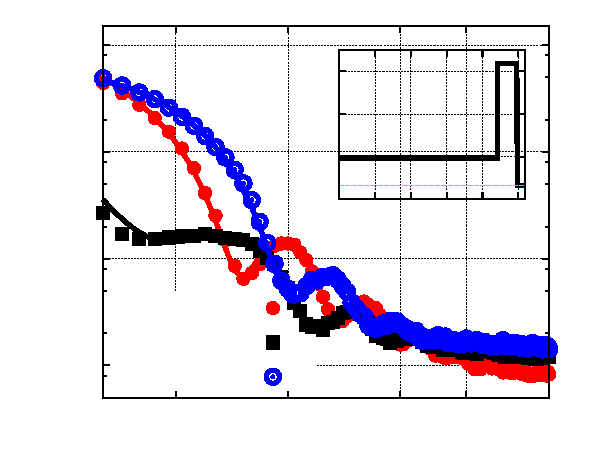
\includegraphics{KiskerSAXSCoreshellFit}}%
    \gplfronttext
  \end{picture}%
\endgroup
